\documentclass[fleqn,11pt]{olplainarticle}
% Use option lineno for line numbers 

\title{Brain - Computer Interfaces - Study Case for Industry Project}

\author[1]{Arturs Elksnis}

\keywords{Brain, Brain - Computer Interface, BCI}

\begin{abstract}
Please provide an abstract of no more than 300 words. Your abstract should explain the main contributions of your article, and should not contain any material that is not included in the main text. 
\end{abstract}

\begin{document}

\flushbottom
\maketitle
\thispagestyle{empty}

\section*{Introduction}
The idea of a Brain - Computer interface (BCI) is decades old, however the latest developments in the field have both opened new possibilities for neurorehabilitation of motor and sensory disabilities and inspired many to imagine applications for healthy people. E.g., the new Neuralink BCI \cite{musk2019integrated} employs more than 1000 electrodes, which closely compares to a hypothetical device in \cite{schalk2008brain} little more than a decade ago. \cite{schalk2008brain} discusses the BCI as an improvement to human efficiency, moreover it talks about much more natural interaction between a machine and a human to the point where the machine feels like an extension of one's body.

While \cite{musk2019integrated} demonstrates a viable engineering solution to fulfill at least some of the speculations in \cite{schalk2008brain}, not enough attention has been given to the social implications of the technology and its emotional impact. After all a technology that promises to extend our physical capabilities must at least introduce profound changes to our social fabric, if not change the whole human experience- much like the introduction of Internet and mobile phones did.

This report therefore analyses potential social and emotional impact of BCI on human society by looking at the social issues experienced by current users of BCIs and by comparing the development of BCI with that of the Internet in the past few decades.

\cite{luz2017enrichment} touches upon the measurement of emotions, which they use to navigate a virtual environment. The measurement of emotions however can serve as an important feedback in end user's satisfaction with BCI.

\cite{kogel2019using} gives a useful summary of many publications that touch upon social aspects of BCI.

gives some insight into the social aspects of the patient-caregiver interaction in medical use cases of BCI.

\section*{Methodology}
The research method employed in this report is purely literature review due to the defined scope of the report. A review of current approach to social aspects of BCI is provided, followed by a few ideas of potential applications. The potential BCI development trajectory is compared to that of the development of Internet. Finally, several social issues are identified along with recommendations to address them.

The PubMed database of  National Center for Biotechnology Information (NCBI) was used as a source for most of the publications and articles reviewed.

\section*{Results}
The idea of BCI controlled closed-loop brain stimulation is met with acceptance among some potential users, while others feel ambivalent or opposed to the concept in principle. Comparing this hypothetical setting with the experiences of the study participants with open-loop brain stimulation, some participants welcomed the prospect of a self-controlled brain stimulation device while other participants maintained reservations. Some study participants expected an improved level of self-expression while others feared a distortion of their sense of self. The new brain stimulation device might also further restrain the user’s sense of accountability, in the case that others would hold the device responsible for their behavior or expressions. Furthermore, this application would require more trust in researchers to keep their data secure and confidential. This last point concerns the issue of meaningful consent. Participants mentioned difficulty in understanding all risks and implications of a closed-loop device both for themselves and for individuals with cognitive impairments. \cite{kogel2019using}

Participants hoped for more independence, self-control, privacy/intimacy, and better communication. Some were concerned about data protection and abuse. Additional concerns raised include the creation of self-transcending human-machine hybrids, as well as the fear for further dependencies, as the BCI necessitates service support and technological maintenance. \cite{kogel2019using}

Breaking the communication bottleneck by adding additional communication channels from the brain to the computer could have profound implications on the way we interact with and benefit from the computer. Additional information may increase the overall communication rate and thus could provide a mechanism to increase human efficiency. Alternatively, augmented awareness about the current state of the brain could make interaction with computers a more natural experience that in the end may not differ from the way we interact with and experience our own body. For example, we might simply focus attention to an Internet link to follow it rather than producing complicated motor commands to move and click a mouse, or we might merely feel that a particular menu selection is not appropriate rather than having to learn the same by reading text on a screen. In summary, the processes that transform our intent into the actions necessary to achieve it could become simpler if we had better access to the current state of the brain. \cite{schalk2008brain}

With relatively modest improvements, brain-computer interfacing technology will become a practical and safe, albeit simple and slow, communication aid. It will thus soon become of interest to the first group of adopters: handicapped individuals who are currently limited for essentially all tasks by their limited communication capacity. For these people, even the modest rates of communication that will initially be achieved should dramatically improve quality of life.\cite{schalk2008brain}

If it becomes possible to design an (ideally non-invasive) interface (see Section 3.3) that can support high performance at an affordable price, brain-computer interfacing technologies will become of interest to the third group of users – most other members of society – that could use these technologies for a wide variety of purposes. At the same time, this new communication capacity will constitute a radical and disruptive innovation that will not be immediately compatible with existing practice and that will evoke change in many complementary processes. It will thus take some time, perhaps a few decades, until this technology has been fully integrated in human societies.

In summary, I expect that, as performance increases and price decreases, brain- computer interfacing technology will become beneficial to an increasing number of individuals, that the direct and indirect effects of its use will become increasingly pervasive, and that the implications on individuals and society will grow in parallel. I thus anticipate that this development of brain-computer interfacing technology will in many ways mirror the development of computers (that addressed the previous bottleneck in human productivity) and of other General-Purpose Technologies (GPTs) [148]. GPTs have been found to have a wide variety of major effects on private and social performance [149]. For example, Information Technology and the Internet have wide applications and productivity-enhancing effects in numerous downstream sectors with high social rates of return that often exceed private rates of return [150, 151], and their dissemination is having a sustained, long-lasting impact on productivity and economic growth. Brain-computer interfacing technology can thus be expected to have a similar profound impact not only on individual, but also on societal performance.
\cite{schalk2008brain}

At the same time, the full potential of direct brain-to-computer communication will only be realized when this technology can benefit most members of society. As soon as interfaces can be built that can interface safely, economically, and concurrently with most of the major systems in the brain, many applications will emerge that will augment our senses and our communication capacities with others and with computers. It will be then that enhanced communication capacities will pervade the fabric of society with a multitude of side effects on many other technologies and processes.\cite{schalk2008brain}

Privacy and Liability in \cite{schalk2008brain}.

\section*{Methods and Materials}

Guidelines can be included for standard research article sections, such as this one.

\section*{Some \LaTeX{} Examples}
\label{sec:examples}

Use section and subsection commands to organize your document. \LaTeX{} handles all the formatting and numbering automatically. Use ref and label commands for cross-references.

\subsection*{Figures and Tables}

Use the table and tabular commands for basic tables --- see Table~\ref{tab:widgets}, for example. You can upload a figure (JPEG, PNG or PDF) using the project menu. To include it in your document, use the includegraphics command as in the code for Figure~\ref{fig:view} below.

\begin{figure}[ht]
\centering
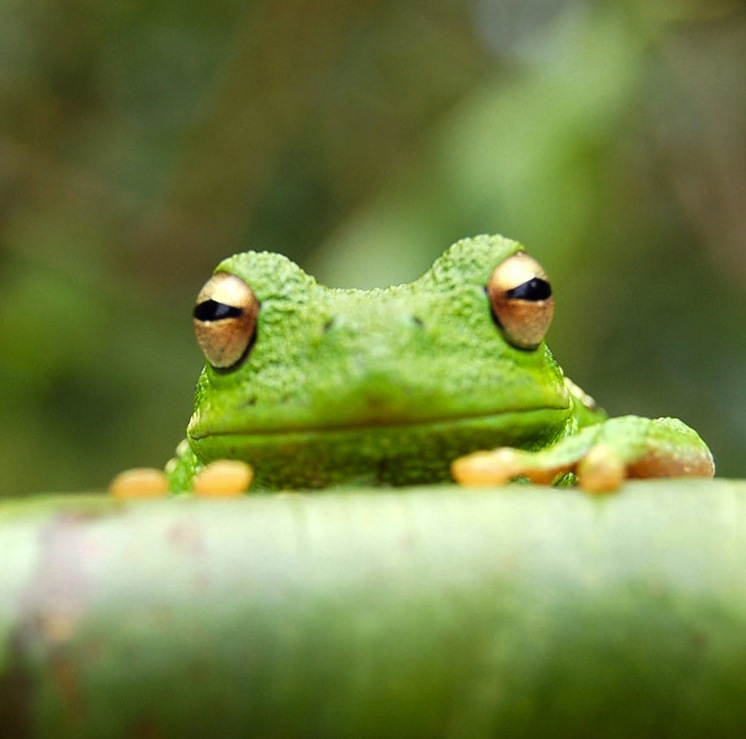
\includegraphics[width=0.7\linewidth]{frog}
\caption{An example image of a frog.}
\label{fig:view}
\end{figure}

\begin{table}[ht]
\centering
\begin{tabular}{l|r}
Item & Quantity \\\hline
Candles & 4 \\
Fork handles & ?  
\end{tabular}
\caption{\label{tab:widgets}An example table.}
\end{table}

\subsection*{Mathematics}

\LaTeX{} is great at typesetting mathematics. Let $X_1, X_2, \ldots, X_n$ be a sequence of independent and identically distributed random variables with $\text{E}[X_i] = \mu$ and $\text{Var}[X_i] = \sigma^2 < \infty$, and let
$$S_n = \frac{X_1 + X_2 + \cdots + X_n}{n}
      = \frac{1}{n}\sum_{i}^{n} X_i$$
denote their mean. Then as $n$ approaches infinity, the random variables $\sqrt{n}(S_n - \mu)$ converge in distribution to a normal $\mathcal{N}(0, \sigma^2)$.

\subsection*{Lists}

You can make lists with automatic numbering \dots

\begin{enumerate}[noitemsep] 
\item Like this,
\item and like this.
\end{enumerate}
\dots or bullet points \dots
\begin{itemize}[noitemsep] 
\item Like this,
\item and like this.
\end{itemize}
\dots or with words and descriptions \dots
\begin{description}
\item[Word] Definition
\item[Concept] Explanation
\item[Idea] Text
\end{description}

\section*{Acknowledgments}

Additional information can be given in the template, such as to not include funder information in the acknowledgments section.

\bibliography{sample}

\end{document}